\documentclass[12pt,a4paper]{article}
\pdfoutput=1

%% template from Klas Eskilson
%% This huge block of usepackages does a lot of things.
%% It makes the text pritty on screens and ensures that you can use some common
%% tools.
%%

\usepackage[utf8]{inputenc}
\usepackage[T1]{fontenc}
% change language to whatever you write in
\usepackage[english]{babel}
\usepackage{amsmath}
\usepackage{lmodern}
\usepackage{listings}
\usepackage{units}
\usepackage{icomma}
\usepackage{color}
\usepackage{graphicx}
\usepackage{multicol,caption}
\usepackage{bbm}
\usepackage{hyperref}
\usepackage{xfrac}
\usepackage{lipsum}
\newcommand{\N}{\ensuremath{\mathbbm{N}}}
\newcommand{\Z}{\ensuremath{\mathbbm{Z}}}
\newcommand{\Q}{\ensuremath{\mathbbm{Q}}}
\newcommand{\R}{\ensuremath{\mathbbm{R}}}
\newcommand{\C}{\ensuremath{\mathbbm{C}}}
\newcommand{\rd}{\ensuremath{\mathrm{d}}}
\newcommand{\id}{\ensuremath{\,\rd}}

%  if you want a page header/footer, use this!
% \usepackage{fancyhdr}
% \pagestyle{fancy}
% \lhead{Left in the header}
% \rhead{Right in the header: \today}

% This creates a nice figure environment that puts the image where you use it,
% and not where LaTeX wants it to be.
\newenvironment{Figure}
  {\par\medskip\noindent\minipage{\linewidth}}
  {\endminipage\par\medskip}

% neat horisontal line
\newcommand{\HRule}{\rule{\linewidth}{0.5mm}}

\begin{document}

\title{The title}
\author{The author}
\date{12-12-12}

%%
%% Use one of these title methods
%%
% \maketitle % simpe latex title
\begin{titlepage}
\begin{center}

% Pre-title
\textsc{TNG022 - Modelling and simulation }\\[0.5cm]

% Title
\HRule \\[0.4cm]
{ \huge \bfseries Modelling and simulating a robot for measuring \\[0.4cm] }

\HRule \\[1.5cm]

% Author and supervisor
\begin{minipage}{0.4\textwidth}
\begin{flushleft} \large
% Author
Group 33\\
Carl Englund\\
\emph{caren083@student.liu.se}
Erik Sandrén\\
\emph{erila135@student.liu.se}
\end{flushleft}
\end{minipage}
\begin{minipage}{0.4\textwidth}
\begin{flushright} \large
% supervisor
Shelley Torgnyson\\
\emph{supervisor@example.com}
\end{flushright}
\end{minipage}

\vfill

% Bottom of the page
{\large Laboration performed: November 27, 2014\\}
{\large Report submitted: \today}

\end{center}
\end{titlepage}

% empty page after title page, ignore this page in the numbering
\newpage\null\thispagestyle{empty}\pagenumbering{gobble}\newpage

\newpage\pagenumbering{arabic} % Arabic page numbers (and reset to 1)

% optional abstract!
\begin{abstract}
\lipsum[4]
\end{abstract}

\newpage

% fairly self-explenatory
\tableofcontents

\newpage

\section{Introduction}
A big part of modelling and simulation revolves around the usage of model descriptions of a system to determine the model's different characteristics.

The purpose of the laboration is to determine the time constant for a DC-motor with two different methods, a simulation of the system and an analytical method. The result of the methods are compared with each other and also with a time constant given by the specifications of the data sheet for the DC-motor. The specifications from the data sheet are achieved by physical measurements by the manufacturer.

The time constant, often denoted with $\tau$, of a system determines how fast it react to changes. The time constant can be retrieved as the time when the system reaches 63\% from the step response's final value. The constant can also be read from the transfer function of a system if given in the form of (\ref{eq:transfer}).

\begin{equation}
\label{eq:transfer}
\frac{K}{\tau s+1}
\end{equation}

\section{Method and materials}
The DC-motor that was used in the laboration was part of a robot arm used for measuring. A schematic picture of the motor was given, see figure \ref{fig:dcmoto}.
The two software packages that were used during the laboration was SIMULINK and 20SIM. The purpose of these softwares are to model electrical and mechanical systems. The softwares can also be used to simulate the models.

As a preparation task for the lab the DC-motor was analyzed and a bond graph was constructed. From the bond graph all the numerical constants were determined and a simple block diagram was constructed for the entire motor. 
\begin{figure}
  \centering
  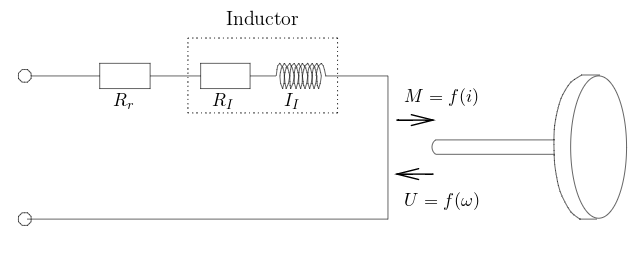
\includegraphics[width=1\linewidth]{schematicdcmotor.png}
  \caption{\emph{Schematic illustration of the DC-motor}}
  \label{fig:dcmoto}
\end{figure}

The system was simulated in 20Sim and Simulink induvidually and with three different simulations. Once for the entire system, electrical part and the mechanical part. All these simulations corresponded with the measured results in the data sheet. The results can be seen in figure X Y and Z. Due to the fact that 20Sims graph tools was found more time consuming then Matlab the results from the simulations were exported from 20Sim to Matlab.
\section{Results}


\section{Discussion}
As seen in the figure X the computed time constant from the simulations, and analitically were the same as the ones denoted in the data sheet. All of this was expected since the systems used in the different methods was identical.

When interpreting the results it can be seen that the electrical system is the fastest while the mechanical system is a bit slower. The entire system is faster than the mechanical system, this is due to the feedback provided from the electrical part.

<--- NEEDS TO MENTION SOMETHING ABOUT THE ANALYTICAL SOLUTION HERE --->

The results retrieved from the data sheet is provided by the manufacturer of the motor and are constructed from physical measurements of the system, but there is no information of how these measurements have been conducted.

\section{Conclusion}
As described in the report computing the time constant analitically can be fast easy and accurate. But depending on the system it may become hard to determine time constant due to the complexity of the time constant equation. When this problem occurs it is easier to use software such as 20Sim or Simulink and compute the time constant using the methods provided in those softwares.

Therefore one needs to carefully analyze the system and decide if it would be more effective to compute the time constant analitically versus computing it using a simulation software such as the ones mentioned before.

% optional bibliography
\begin{thebibliography}{99}

\end{thebibliography}

\end{document}